\documentclass[t]{beamer}
\usetheme[deutsch]{KIT}
\setbeamercovered{transparent}
\setbeamertemplate{navigation symbols}{}

\KITfoot{Tutoriumsmaterial von Michael Fuerst}
\usepackage[utf8]{inputenc}
\usepackage{amsmath}
\usepackage{ifthen}
\usepackage{amssymb}
\usepackage{tikz}
\usepackage{ngerman}
\usepackage[normalem]{ulem}
\usepackage{stmaryrd}
\usetikzlibrary{automata}
\usenavigationsymbols


\title{Theoretische Grundlagen der Informatik}
\subtitle{Tutorium}
\author{Michael Fuerst}

\institute[IKS]{Institut für Theoretische Informatik}

\TitleImage[height=\titleimageht]{images/tmaschine.png}

\newcommand{\N}{\ensuremath{\mathbb{N}}}
\newcommand{\M}{\ensuremath{\mathcal{M}}}
\newcommand{\classP}{\ensuremath{\mathcal{P}}}
\newcommand{\classNP}{\ensuremath{\mathcal{NP}}}
\newcommand{\co}{\ensuremath{\mathsf{co\text{-}}}}
\newcommand{\pot}{\ensuremath{\mathcal{P}}}
\newcommand{\abs}[1]{\ensuremath{\left\vert #1 \right\vert}}
\newcommand{\menge}[2]{\ensuremath{\left\lbrace #1 \,\middle\vert\, #2 \right\rbrace}}
\newcommand{\ducttape}[1]{\vspace{#1}}
\newcommand{\neglit}[1]{\overline{#1\vphantom{x^a}}}
\newcommand{\recipe}{\raisebox{-.3cm}{
\includegraphics[scale=.15]{images/chefs-cap.png}}\hspace{0.2cm}}
\newcommand{\opt}[1]{\ensuremath{\text{OPT}(#1)}}
\newcommand{\A}[1]{\ensuremath{\mathcal{A}(#1)}}
\renewcommand{\O}[1]{\ensuremath{\mathcal{O}(#1)}}
\newcommand{\msout}[1]{\text{\sout{\ensuremath{#1}}}}

\newcommand{\invincible}{\setbeamercovered{invisible}} %  "Yesss! I am invincible!!" (Boris Grishenko)
\newcommand{\vincible}{\setbeamercovered{transparent}}
\renewcommand{\solution}[1]{\invincible \pause #1 \vincible}
\newcommand{\micropause}{\\[8pt]}

% \@ifundefined{tikzset}{}{\tikzset{initial text=}} % Text "start" bei Startknoten unterdrücken
\tikzstyle{every node}=[thick]
\tikzstyle{every line}=[thick]

\newcommand{\tutnr}[1]{
  \subtitle{Tutorium #1}
	\begin{frame}
		\maketitle
	\end{frame}
}

\newcommand{\uebnr}[1]{
  \subtitle{Anmerkungen zum #1. Übungsblatt}
	\begin{frame}
		\maketitle
	\end{frame}
}

\begin{document}

\tutnr{11}

\section{Chomsky-Normalform}
\subsection{Chomsky-Normalform}
\frame{
\frametitle{Chomsky-Normalform}
Der Cocke-Younger-Kasami-Algorithmus (CYK) löst das Wortproblem für kontextfreie Sprachen (CH-2) in $\O{n^3}$.
Um CYK anzuwenden, muss die gegebene Grammatik erst in Chomsky-Normalform gebracht werden. Das ist für jede CH-2-Grammatik möglich.
\
\begin{exampleblock}{Chomsky-Normalform}
Eine CH-2-Grammatik \textit{G} $= (\Sigma,\mathcal{V,S,R) }$ ist in Chomsky-Normalform,  wenn jede Produktion aus $\mathcal{R}$ eine der folgenden Formen hat:
\begin{itemize}
\item  $A \rightarrow BC$
\item  $A \rightarrow a$
\end{itemize}
Wobei gilt $A,B,C\in\mathcal{V}$ und $a \in \Sigma$.
Um das leere Wort in der Sprache zu erlauben, lässt sich die Grammatik leicht mit neuem Startsymbol $S'$ ergänzen mit der Regel $$ S' \rightarrow S \mid \varepsilon $$
\end{exampleblock}
}


%\subsection{Umwandlung in Chomsky-Normalform}
\frame{
\frametitle{Umwandlung in Chomsky-Normalform}
\begin{enumerate}
\item Für alle $\textcolor{red}{a} \in \Sigma$ und für alle Produktionen, auf deren rechter Seite $\textcolor{red}{a}$ vorkommt 
(außer für $V  \rightarrow \textcolor{red}{a}$, mit $V \in\mathcal{V}$),
wird jedes Vorkommen von $\textcolor{red}{a}$ durch ein \emph{neues} Nichtterminalsymbol $\textcolor{blue}{A}$ ersetzt
%(und $A$ in die Variablenmenge aufgenommen)
und die Produktion $\textcolor{blue}{A} \rightarrow \textcolor{red}{a}$ wird hinzugefügt.
\end{enumerate}

\begin{exampleblock}{Umwandlungsbeispiel (Schritt 1 von 4)}
\begin{columns}[c]
\begin{column}{0.3\textwidth}
\begin{align*}
\mathcal{S} &\rightarrow XY\\
X &\rightarrow \textcolor{red}{a}X\textcolor{red}{b} \mid Z \mid \varepsilon\\
Y &\rightarrow \textcolor{red}{cc}Y \mid \varepsilon\\
Z &\rightarrow X\\
\end{align*}
\end{column}
%
\
\begin{column}{0.05\textwidth}
$\Rightarrow$
\end{column}
%
\begin{column}{0.3\textwidth}
\begin{align*}
\mathcal{S} &\rightarrow XY\\
X &\rightarrow \textcolor{blue}{A}X\textcolor{blue}{B} \mid Z \mid \varepsilon\\
Y &\rightarrow \textcolor{blue}{CC}Y \mid \varepsilon\\
Z &\rightarrow X\\
\textcolor{blue}{A} &\rightarrow \textcolor{red}{a}\\
\textcolor{blue}{B} &\rightarrow \textcolor{red}{b}\\
\textcolor{blue}{C} &\rightarrow \textcolor{red}{c}\\
\end{align*}
\end{column}
\end{columns}
\end{exampleblock}
}

\frame{
\frametitle{Umwandlung in Chomsky-Normalform}
\begin{enumerate}
\setcounter{enumi}{1}
\item
Für Produktionen mit mehr als zwei
Variablen rechts werden \textcolor{blue}{ \emph{neue} Nichterminale} eingeführt
und dazu \textcolor{blue}{passende Produktionen} hinzugefügt.
\end{enumerate}

\begin{exampleblock}{Umwandlungsbeispiel (Schritt 2 von 4)}
\begin{columns}[c]
\begin{column}{0.3\textwidth}
\begin{align*}
\mathcal{S} &\rightarrow XY\\
X &\rightarrow \textcolor{red}{AXB} \mid Z \mid \varepsilon \\
Y &\rightarrow \textcolor{red}{CCY} \mid \varepsilon \\
Z &\rightarrow X\\
A &\rightarrow a\\
B &\rightarrow b\\
C &\rightarrow c\\
\end{align*}
\end{column}
%
\
\begin{column}{0.05\textwidth}
$\Rightarrow$
\end{column}
%
\begin{column}{0.3\textwidth}
\begin{align*}
\mathcal{S} &\rightarrow XY\\
X &\rightarrow \textcolor{blue}{FB} \mid Z \mid \varepsilon \\
Y &\rightarrow \textcolor{blue}{GY} \mid \varepsilon \\
Z &\rightarrow X\\
\textcolor{blue}{F} &\rightarrow \textcolor{blue}{AX}\\
\textcolor{blue}{G} &\rightarrow \textcolor{blue}{CC}\\
A &\rightarrow a\\
B &\rightarrow b\\
C &\rightarrow c\\
\end{align*}
\end{column}
\end{columns}
\end{exampleblock}
}

\begin{frame}
\frametitle{Umwandlung in Chomsky-Normalform}
\begin{enumerate}
\setcounter{enumi}{2}
\item Entfernen von Produktionen der Form $\textcolor{red}{V} \rightarrow \textcolor{red}{\varepsilon}$
f"ur $V \in \mathcal{V}, v \neq \mathcal{S}$ \\ $\Rightarrow$ "`Vorwegnahme"' dieser Produktionen: Für jede Produktion mit einem der obigen $V$
auf der rechten Seite wird eine \textcolor{blue}{neue Produktion} ohne dieses $V$ hinzugefügt.
\end{enumerate}

\begin{exampleblock}{Umwandlungsbeispiel (Schritt 3 von 4)}
\ducttape{-0.25cm}
\begin{columns}[c]
\begin{column}{0.3\textwidth}
\begin{align*}
\mathcal{S} &\rightarrow XY\\
\textcolor{red}{X} &\rightarrow FB \mid Z \mid \textcolor{red}{\varepsilon}\\
\textcolor{red}{Y} &\rightarrow GY \mid \textcolor{red}{\varepsilon}\\
Z &\rightarrow X\\
F &\rightarrow AX\\
G &\rightarrow CC\\
A &\rightarrow a, B \rightarrow b, C \rightarrow c\\
\end{align*}
\end{column}
%
\
\begin{column}{0.05\textwidth}
$\Rightarrow$
\end{column}
%
\begin{column}{0.3\textwidth}
\begin{align*}
\textcolor{red}{\mathcal{S}} &\rightarrow XY \mid \textcolor{blue}{X} \mid  \textcolor{blue}{Y} \mid \textcolor{blue}{\varepsilon}\\
\textcolor{red}{X} &\rightarrow FB \mid Z \mid \textcolor{blue}{\msout{\varepsilon}}\\
\textcolor{red}{Y} &\rightarrow GY \mid \textcolor{blue}{G}\\
\textcolor{red}{Z} &\rightarrow X\mid \textcolor{blue}{\msout{\varepsilon}}\\
F &\rightarrow AX \mid \textcolor{blue}{A}\\
G &\rightarrow CC\\
A &\rightarrow a, B \rightarrow b, C \rightarrow c\\
\end{align*}
\end{column}
\end{columns}
\end{exampleblock}
\end{frame}



\frame{
\frametitle{Umwandlung in Chomsky-Normalform}
\begin{enumerate}
\setcounter{enumi}{3}
\item
Für Produktionen mit einer Variablen rechts werden Zyklen gesucht, 
für gefundene Zyklen werden alle Vorkommnisse aller Variablen des Zyklus durch einen Repräsentanten ausgetauscht. Danach werden triviale Produktionen entfernt.
\end{enumerate}

\begin{exampleblock}{Umwandlungsbeispiel (Schritt 4a von 4)}
\begin{columns}[c]
\begin{column}{0.3\textwidth}
\begin{align*}
\mathcal{S} &\rightarrow XY \mid X \mid Y \mid \varepsilon \\
\textcolor{red}{X} &\rightarrow FB \mid \textcolor{red}{Z} \\
Y &\rightarrow GY \mid G \\
\textcolor{red}{Z} &\rightarrow \textcolor{red}{X}\\
F &\rightarrow AX \mid A\\
G &\rightarrow CC\\
A &\rightarrow a, B \rightarrow b, C \rightarrow c\\
\end{align*}
\end{column}
%
\
\begin{column}{0.05\textwidth}
$\Rightarrow$
\end{column}
%
\begin{column}{0.3\textwidth}
\begin{align*}
\mathcal{S} &\rightarrow XY \mid X \mid Y \mid \varepsilon \\
\textcolor{blue}{X} &\rightarrow FB \mid \msout{\textcolor{blue}{X}} \\
Y &\rightarrow GY \mid G\\
\msout{\textcolor{blue}{X}} &\rightarrow \msout{\textcolor{blue}{X}}\\
F &\rightarrow AX\\
G &\rightarrow CC\\
A &\rightarrow a, B \rightarrow b, C \rightarrow c\\
\end{align*}
\end{column}
\end{columns}
\end{exampleblock}
}

\frame{
\frametitle{Umwandlung in Chomsky-Normalform}
\begin{enumerate}
\setcounter{enumi}{3}
\item
Alle Regeln, die rechts eine einzelne Variable haben, werden durch "`Vorziehen"' der Regeln eliminiert.

Außerdem wird ein neues Startsymbol eingeführt, falls eine Regel $\mathcal{S} \rightarrow \varepsilon$ existiert.
\end{enumerate}

\begin{exampleblock}{Umwandlungsbeispiel (Schritt 4b von 4)}
\ducttape{-0.4cm}
\begin{columns}[c]
\begin{column}{0.3\textwidth}
\begin{align*}
\mathcal{S} &\rightarrow XY \mid \textcolor{red}{X} \mid  \textcolor{red}{Y} \mid \textcolor{red}{\varepsilon}\\
X &\rightarrow FB\\
Y &\rightarrow GY \mid \textcolor{red}{G}\\
F &\rightarrow AX\\
G &\rightarrow CC\\
A &\rightarrow a\\
B &\rightarrow b\\
C &\rightarrow c\\
\end{align*}
\end{column}
%
\
\begin{column}{0.05\textwidth}
$\Rightarrow$
\end{column}
%
\begin{column}{0.3\textwidth}
\begin{align*}
\textcolor{blue}{\mathcal{S}} & \rightarrow \textcolor{blue}{\mathcal{S'} \mid \varepsilon} \\
\mathcal{S'} &\rightarrow XY \mid \textcolor{blue}{FB} \mid \textcolor{blue}{GY} \mid \textcolor{blue}{CC}\\
X &\rightarrow FB \\
Y &\rightarrow GY \mid \textcolor{blue}{CC} \\
F &\rightarrow AX\\
G &\rightarrow CC\\
A &\rightarrow a\\
B &\rightarrow b\\
C &\rightarrow c\\
\end{align*}
\end{column}
\end{columns}
\end{exampleblock}
}

\begin{frame}
\frametitle{Aufgabe}
Sei $G=(\Sigma,V,S,R)$ die CH-2-Grammatik mit $\Sigma = \{a,b\}$, $V=\{A,B,C,D,E,S\}$ und der folgenden Regelmenge $R$:
\begin{eqnarray*}
S & \rightarrow & A \;|\; aAa  \;|\; bBb  \;|\; \varepsilon \\
A & \rightarrow & C \;|\; a \\
B & \rightarrow & C \;|\; b \\
C & \rightarrow & CDE \;|\; \varepsilon \\
D & \rightarrow & A \;|\; B \;|\; ab \\
E & \rightarrow & S
\end{eqnarray*}
Bestimme eine Grammatik $G'$ für $L(G)$ in Chomsky-Normalform.
\end{frame}

\section{CYK}
\subsection{Not CMYK!}

\frame{
\frametitle{CYK Überblick}
CYK ist ein Algorithmus, um das Wortproblem in CH-2 zu lösen. Um den Algorithmus anzuwenden, muss eine Grammatik in Chomsky-Normalform vorliegen.\\
Grundidee zur Überprüfung eines Wortes der Länge $n$:
\begin{itemize}
\item Wir betrachen $V_{i,j} = $ Menge der Nichtterminale, aus denen das Teilwort der Position $i$ bis $j$ abgeleitet werden kann
\item Die Frage, ob $V_{i,j}$ ableitbar ist, lässt sich entscheiden durch Betrachten aller möglichen $V_{i,k}$ und $V_{k+1,j}$
\item $V_{i,i}$ sind trivial
\item Bottom-up lässt sich dadurch $V_{1,n}$ berechnen
\item Ist $S \in V_{1,n}$, so lässt sich das Wort ableiten
\end{itemize}
}

\frame{
\frametitle{CYK}
Gegeben sei die Grammatik \textit{G} $= \mathcal{(T,V,}S\mathcal{,P) }$  mit den folgenden Produktionen aus $\mathcal{P}$:
\begin{align*}
S & \rightarrow AX \mid AB \\
X &\rightarrow SB \mid AB \\
A &\rightarrow a\\
B &\rightarrow b\\
\end{align*}
\begin{enumerate}
	\item Lässt sich der CYK-Algorithmus auf $G$ anwenden?
	\item Ist das Wort $aaabbb$ in der Sprache $\mathcal{L}(\textit{G})$?
\end{enumerate}
}
\section{Pumping Lemma und Ogdens Lemma}
\subsection{Pumping Lemma für kontextfreie Sprachen}
\begin{frame}
\frametitle{Pumping-Lemma für kontextfreie Sprachen}
\begin{exampleblock}{Lemma}
Für jede kontextfreie Sprache $L$ gibt es eine Konstante $n \in \mathbb{N}$,
so dass sich jedes Wort $z \in L$ mit $|z| \geq n$ so als
$$ z = uvwxy $$
schreiben lässt, dass
\begin{itemize}
\item $|vx| \geq 1$,
\item $|vwx| \leq n$ und
\item für alle $i \geq 0$ das Wort $uv^iwx^iy \in L$ ist.
\end{itemize}
\end{exampleblock}
\end{frame}

\begin{frame}
\frametitle{Beweisidee}
\begin{itemize}
\item Jeder Knoten im Ableitungsbaum (wie wir ihn in CYK sehen) steht für ein Nichtterminalsymbol
\item Ab einer gewissen Höhe des Baumes (bzw. Länge des Wortes) muss ein Nichtterminal im Baum mehrmals in einer Reihe vorkommen
\item Man kann also aus einem Nichtterminalsymbol dasselbe Symbol wieder ableiten
\item Da das Wort durch jede Ableitung (außer zu Terminalsymbolen) länger wird, gibt es eine "`Schleife"' beim Ableiten
\item Diese Schleife kann man also "`pumpen"', also beliebig oft (oder auch gar nicht) durchlaufen
\end{itemize}
\end{frame}

\begin{frame}
	\frametitle{Beweisidee}
	\begin{figure}[H]
		\centering
		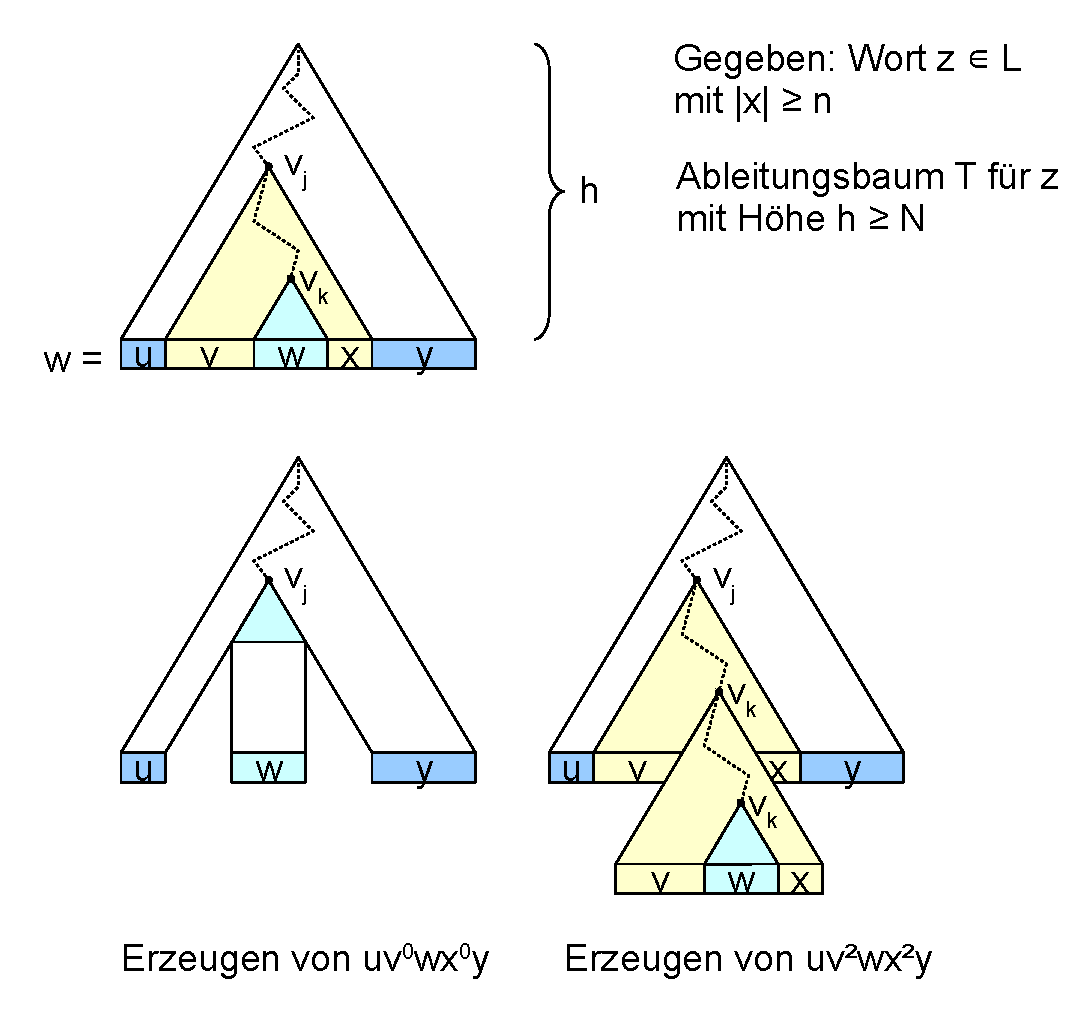
\includegraphics[scale=0.5]{images/pumping}
	\end{figure}
\end{frame}

\subsection{Ogdens Lemma}
\begin{frame}
\frametitle{Ogdens Lemma für kontextfreie Sprachen}
\begin{exampleblock}{Lemma}
Für jede kontextfreie Sprache $L$
gibt es eine Konstante $n \in \mathbb{N}$, so dass für jedes Wort $z \in L$ mit $|z| \geq n$ gilt:\\
Wenn wir in $z$ mindestens $n$ Buchstaben markieren, so lässt sich $z$ so als $z = uvwxy$ schreiben, dass
\begin{itemize}
\item von den mindestens $n$ markierten Buchstaben
\begin{itemize}
\item mindestens einer zu $vx$ gehört und
\item höchstens $n$ zu $vwx$ gehören und
\end{itemize}
\item für alle $i \geq 0$ das Wort $uv^iwx^iy \in L$ ist.
\end{itemize}
\end{exampleblock}
\end{frame}

\begin{frame}
\frametitle{Zu Ogden und Pumping ...}
\begin{itemize}
\item Anwendung genau wie "`altes"' Pumping Lemma
\item Wird verwendet, um zu zeigen dass eine Sprache nicht kontextfrei ist
\item Dazu: Kontraposition bilden und folgern, dass Sprache nicht kontextfrei
\end{itemize}
\end{frame}

\begin{frame}
\frametitle{Aufgabe}

Zeige, dass folgende Sprachen nicht kontextfrei sind:

\begin{enumerate}
  \item $L_1 = \{w \in \{a, b, c\}^*: |w|_a = |w|_b = |w|_c\}$,
	wobei $|w|_x$ für die Häufigkeit des
	Buchstabens $x$	im Wort $w$ stehe.
  \item $L_2 = \{a^ib^ic^j \mid j \leq i\}$
  \item $L_3=\{a^ib^jc^id^j \mid i,j \geq 1 \}$

\end{enumerate}
\end{frame}

\section{Schluss}
\subsection{Aus!}
\begin{frame}
\frametitle{Bis zum nächsten Mal!}
\only<1>{
	\begin{figure}[H]
		
\includegraphics[height= 0.8\textheight]{images/grandma}

        \textit{\scriptsize{http://twitter.com/herpderpedia}}
	\end{figure}
}

\only<2>{
	\begin{figure}[H]
		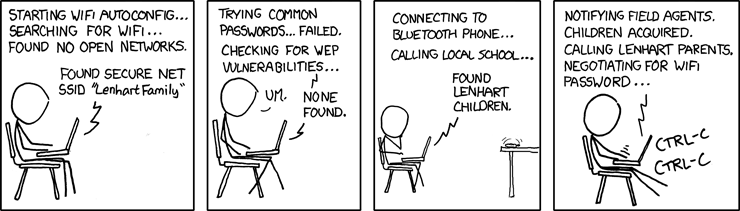
\includegraphics[width= \textwidth]{images/xkcd_416}
		
		\textit{\scriptsize{I hear this is an option in the latest Ubuntu release.}}
		
	\end{figure}
}
\end{frame}

\frame{
  \frametitle{Lizenzen}
  \center
  
\includegraphics[width=2em]{images/by}
  
\includegraphics[width=2em]{images/cc}
  
\includegraphics[width=2em]{images/sa}
  \\
  {\tiny

Dieses Werk ist unter einem ``Creative Commons Namensnennung-Weitergabe unter gleichen Bedingungen 3.0 Deutschland``-Lizenzvertrag lizenziert. Um eine Kopie der Lizenz zu erhalten, gehen Sie bitte zu \href{http://creativecommons.org/licenses/by-sa/3.0/de/}{http://creativecommons.org/licenses/by-sa/3.0/de/} oder schreiben Sie an Creative Commons, 171 Second Street, Suite 300, San Francisco, California 94105, USA.\\
  \vspace{1cm}
  Davon ausgenommen sind das Titelbild, welches aus der März-April 2002 Ausgabe von American Scientist erschienen ist und ohne Erlaubnis verwendet wird, sowie das KIT Beamer Theme. Hierfür gelten die Bestimmungen der jeweiligen Urheber.
  \vspace{1cm}
  \\ 
  }
  %Habe hier die Reihenfolge etwas umgestellt, weil die Formatierung bei mir komisch aussah. 
  %Wenn es bei dir anders ist, kannst du es auch wieder zurückändern, dann haben wir unterschiedliche Kompilieroptionen
}

\end{document}
